        We prove that for any homothet $C$ with two points
        $\pa,\pb\in \PS$ on its boundary, there is a path between $\pa$
        and $\pb$ in $\restrictY{\DT}{C}$, and \lemref{shrink:shrank} will
        immediately imply the general statement. The proof is by induction
        over the number $m$ of points of $\PS$ in the interior of $C$. If
        $m=0$ then $C$ contains no points of $\PS$ in its interior, and
        thus $\pa \pb$ is an edge of the Delaunay triangulation, as $C$
        testifies.
        
        \begin{figure}[h]
                \phantom{}\hfill%
                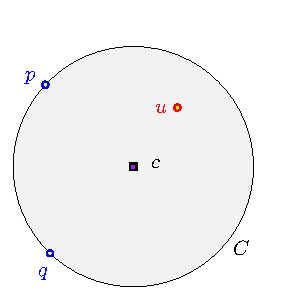
\includegraphics[page=1]{../figs/shrink}%
                \hfill%
                \includegraphics[page=2]{../figs/shrink}%
                \hfill%
                \includegraphics[page=3]{../figs/shrink}%
                \hfill%
                \phantom{}%
                \caption{An illustration of the proof of
                        \clmref{c:t:connected} in the case that $C$ is a disk.}
                \figlab{shrink}
        \end{figure}
        
        Otherwise, let $\pc\in \PS$ be a point in the interior of
        $C$. From \lemref{shrink:shrank} we get that there exists a
        homothet $C'$ of $C$ with $C'\subseteq C$, such that $\pa$ and
        $\pc$ lie on the boundary of $C'$ Thus, by induction, there is
        a path $\gamma'$ between $\pa$ and $\pc$ in
        $\restrictY{\DT}{C'} \subseteq \restrictY{\DT}{C}$. Similarly,
        there must be a homothet $C''$, that gives rise to a path
        $\gamma''$ between $\pc$ and $\pb$, and concatenating the two
        paths results in a path between $\pa$ and $\pb$ in
        $\restrictY{\DT}{C}$.
